\setauthor{\firstauthor}

\subsubsection{UI-Frameworks}
\label{sec:ui-frameworks}

Für die Gestaltung der Benutzeroberfläche von LearnHub wurden drei verbreitete
UI-Frameworks evaluiert: \textbf{Bootstrap}, \textbf{Tailwind CSS} und
\textbf{Angular Material}.
Die Wahl des Frameworks beeinflusst maßgeblich die Entwicklungsgeschwindigkeit,
die visuelle Konsistenz sowie die langfristige Wartbarkeit einer
Webanwendung.
Zur Bewertung wurden die Frameworks anhand identischer UI-Elemente –
konkret eines Eingabeformulars – gegenübergestellt, da Formulare in
LearnHub (Fragenerstellung, Maturathemenupload) eine zentrale Rolle einnehmen.

\paragraph{Bootstrap}


Bootstrap ist ein Open-Source-Frontend-Framework, das 2011 von Twitter
veröffentlicht wurde und auf einem 12-Spalten-Grid-System sowie
vordefinierten CSS-Komponenten basiert~\cite{bootstrap2023docs}.
Gestaltungselemente wie Buttons, Formulare und Navigationsleisten werden
durch das Hinzufügen vordefinierter CSS-Klassen direkt im HTML-Markup
aktiviert, ohne dass eigener CSS-Code notwendig ist.

Listing~\ref{lst:bootstrap-form} zeigt die Implementierung eines
Eingabeformulars in Bootstrap.

\begin{lstlisting}[style=htmlstyle, caption={Eingabeformular mit Bootstrap},
                   label={lst:bootstrap-form}]
<form>
  <div class="mb-3">
    <label for="subject" class="form-label">Fach</label>
    <input type="text"
           class="form-control"
           id="subject"
           placeholder="z.B. Mathematik">
  </div>
  <div class="mb-3">
    <label for="topic" class="form-label">Themenpool</label>
    <select class="form-select" id="topic">
      <option>Algebra</option>
      <option>Analysis</option>
    </select>
  </div>
  <button type="submit" class="btn btn-primary">
    Speichern
  </button>
</form>
\end{lstlisting}

 \begin{figure}[H]
   \centering
   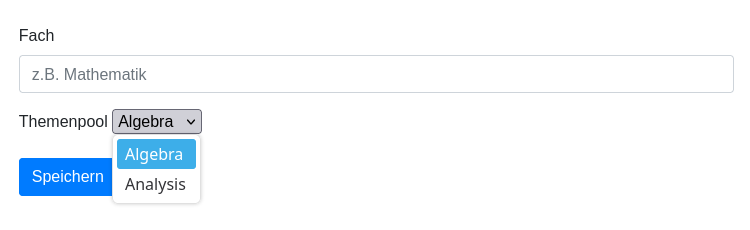
\includegraphics[width=0.8\textwidth]{./pics/bootstrap_form.png}
   \caption{Darstellung des Formulars mit Bootstrap (Standard-Theme)}
   \label{fig:bootstrap-form}
 \end{figure}

Das resultierende Formular zeichnet sich durch ein einheitliches Erscheinungsbild
aus: abgerundete Eingabefelder mit einem blauen
Primär-Button, die dem standardisierten Bootstrap-Design entsprechen.
Dieses visuelle Muster ist in zahlreichen Webanwendungen verbreitet und
für Entwickler:innen unmittelbar erkennbar~\cite{bootstrap2023docs}.

\textbf{Vorteile:}
\begin{itemize}
  \item Geringe Einarbeitungszeit durch standardisierte Klassen
  \item Umfangreiche Dokumentation und große Entwickler:innen-Community
  \item Responsives 12-Spalten-Grid ohne zusätzlichen CSS-Aufwand
  \item Vorgefertigte Komponenten (Modals, Dropdowns, Cards)
\end{itemize}

\textbf{Nachteile:}
\begin{itemize}
  \item Designs wirken ohne individuelle Anpassung generisch~
  \item Erhöhte HTML-Komplexität durch viele Klassen-Bezeichner
  \item Bundle-Size steigt bei Einbindung nicht genutzter Komponenten
\end{itemize}

\paragraph{Tailwind CSS}

Tailwind CSS ist ein \textit{Utility-First}-Framework, das 2017 von Adam
Wathan entwickelt wurde~\cite{tailwind2023docs}.
Im Gegensatz zu komponentenbasierten Frameworks wie Bootstrap stellt
Tailwind keine vordefinierten Komponenten bereit.
Stattdessen werden visuelle Eigenschaften durch die direkte Kombination
einzelner Hilfsklassen (\textit{Utility Classes}) im HTML-Markup definiert.
Durch einen integrierten Purge-Mechanismus werden im Produktions-Build
ausschließlich tatsächlich verwendete Klassen in die finale CSS-Datei
aufgenommen, was die Bundle-Size erheblich reduziert~\cite{tailwind2023docs}.

Listing~\ref{lst:tailwind-form} zeigt das identische Formular,
implementiert mit Tailwind CSS.

\begin{lstlisting}[style=htmlstyle, caption={Eingabeformular mit Tailwind CSS},
                   label={lst:tailwind-form}]
<form class="space-y-4">
  <div>
    <label class="block text-sm font-medium text-gray-700">
      Fach
    </label>
    <input type="text"
      class="mt-1 block w-full rounded-md border border-gray-300
             shadow-sm focus:border-indigo-500 focus:ring-indigo-500
             sm:text-sm px-3 py-2"
      placeholder="z.B. Mathematik">
  </div>
  <div>
    <label class="block text-sm font-medium text-gray-700">
      Themenpool
    </label>
    <select class="mt-1 block w-full rounded-md border border-gray-300
                   shadow-sm focus:border-indigo-500 sm:text-sm
                   px-3 py-2">
      <option>Algebra</option>
      <option>Analysis</option>
    </select>
  </div>
  <button class="bg-indigo-600 text-white px-4 py-2 rounded-md
                 hover:bg-indigo-700 transition-colors duration-200
                 text-sm font-medium">
    Speichern
  </button>
</form>
\end{lstlisting}


 \begin{figure}[H]
   \centering
   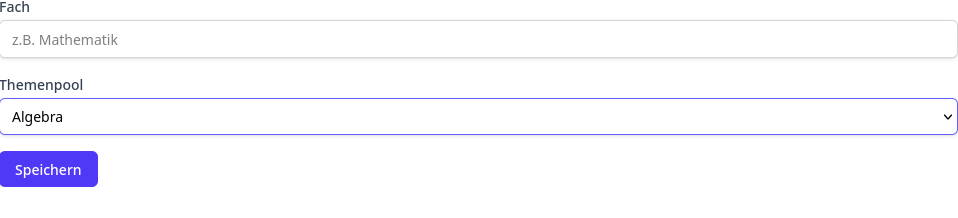
\includegraphics[width=0.8\textwidth]{./pics/tailwind_form.png}
   \caption{Darstellung des Formulars mit Tailwind CSS}
   \label{fig:tailwind-form}
 \end{figure}

Der direkte Vergleich mit dem Bootstrap-Formular verdeutlicht einen
wesentlichen Unterschied: Während Bootstrap ein festgelegtes visuelles
Design vorgibt, entsteht das Erscheinungsbild bei Tailwind ausschließlich
durch die gewählte Kombination der Utility-Klassen.
Dies ermöglicht eine hohe visuelle Differenzierung, erhöht jedoch den
initialen Implementierungsaufwand pro Komponente~\cite{tailwind2023docs}.

\textbf{Vorteile:}
\begin{itemize}
  \item Maximale Designfreiheit ohne separate CSS-Datei
  \item Sehr geringe Bundle-Size durch Purge-Mechanismus im Build
  \item Konsistente Design-Tokens (Farben, Abstände, Schatten)
        über das gesamte Projekt
\end{itemize}

\textbf{Nachteile:}
\begin{itemize}
  \item Steile Lernkurve, insbesondere für Entwickler:innen ohne
        Vorerfahrung
  \item Kein vorgefertigtes Komponentensystem
  \item Verringerte HTML-Lesbarkeit durch lange Klassenketten
\end{itemize}
\setauthor{\firstauthor}
\paragraph{Angular Material}

Angular Material ist eine von Google entwickelte Komponentenbibliothek,
die auf dem Material-Design-Designsystem basiert und speziell für das
Angular-Framework konzipiert wurde~\cite{angularmaterial2023docs}.
Im Unterschied zu Bootstrap und Tailwind CSS werden keine CSS-Klassen
vergeben; stattdessen stehen vollständige Angular-Komponenten als
TypeScript-Module bereit, die als HTML-Tags eingesetzt werden
(\texttt{<mat-form-field>}, \texttt{<mat-button>} etc.).
Ab Angular~17 wird das klassische \texttt{NgModule}-Muster durch
Standalone Components ersetzt: Jede Komponente deklariert ihre
Abhängigkeiten direkt im \texttt{imports}-Array des
\texttt{@Component}-Dekorators~\cite{angularmaterial2023docs}.
Listing~\ref{lst:angularmaterial-ts} zeigt den erforderlichen
Komponenten-Import, Listing~\ref{lst:angularmaterial-html} das zugehörige
Template.

\begin{lstlisting}[style=tsstyle,
                   caption={Standalone Component mit Angular Material (app.ts)},
                   label={lst:angularmaterial-ts}]
import { Component } from '@angular/core';
import { FormsModule } from '@angular/forms';
import { MatFormFieldModule }
  from '@angular/material/form-field';
import { MatInputModule }
  from '@angular/material/input';
import { MatSelectModule }
  from '@angular/material/select';
import { MatButtonModule }
  from '@angular/material/button';

@Component({
  selector: 'app-root',
  standalone: true,
  imports: [
    FormsModule,
    MatFormFieldModule,
    MatInputModule,
    MatSelectModule,
    MatButtonModule,
  ],
  templateUrl: './app.html',
})
export class App {
  fach = '';
  thema = '';
}
\end{lstlisting}

\begin{lstlisting}[style=htmlstyle,
                   caption={Eingabeformular mit Angular Material},
                   label={lst:angularmaterial-html}]
<div>
  <mat-form-field appearance="outline">
    <mat-label>Fach</mat-label>
    <input matInput placeholder="z.B. Mathematik"
           [(ngModel)]="fach" name="fach">
  </mat-form-field>
  <mat-form-field appearance="outline">
    <mat-label>Themenpool</mat-label>
    <mat-select [(ngModel)]="thema">
      <mat-option value="algebra">Algebra</mat-option>
      <mat-option value="analysis">Analysis</mat-option>
    </mat-select>
  </mat-form-field>
  <button mat-raised-button color="primary">
    Speichern
  </button>
</div>
\end{lstlisting}

%
\begin{figure}[H]
\centering
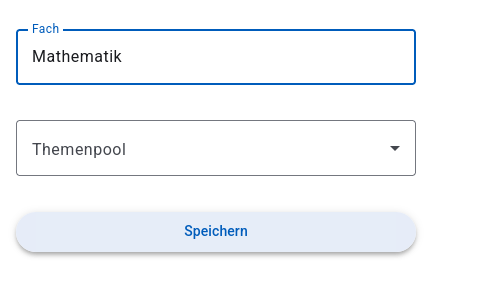
\includegraphics[width=0.6\textwidth]{./pics/angularmaterial_form.png}
\caption{Darstellung des Formulars mit Angular Material}
\label{fig:angularmaterial-form}
\end{figure}

Angular Material zeichnet sich durch das charakteristische
\textit{Floating-Label}-Verhalten aus: Das Label schwebt beim
Fokussieren des Eingabefelds nach oben, was dem Material-Design-Standard
von Google entspricht.
Barrierefreiheitsstandards (ARIA) sowie die native Integration mit
Angular Reactive Forms sind ohne zusätzliche Konfiguration gewährleistet~\cite{angularmaterial2023docs}.

\textbf{Vorteile:}
\begin{itemize}
  \item Native Integration mit Angular 
  \item Einheitliches, professionelles Erscheinungsbild
\end{itemize}

\textbf{Nachteile:}
\begin{itemize}
  \item Eingeschränkte visuelle Anpassbarkeit
        (Material-Design-Erscheinungsbild stark vorgegeben)
  \item Höherer initialer Konfigurationsaufwand durch das Theming-System
  \item Größere Bundle-Size durch Komponentenstruktur
\end{itemize}

\setauthor{\firstauthor}
\paragraph{Vergleich und Technologieentscheidung}

Auf Basis der technischen Analyse sowie der verfügbaren Erfahrung des
Entwicklungsteams wurde \textbf{Bootstrap} als UI-Framework für LearnHub
gewählt.

Der ausschlaggebende Faktor war der Entwicklungsaufwand: Bootstrap war
im Team bereits aus dem Schulunterricht bekannt und wurde in kleineren
Projekten eingesetzt. Dadurch entfiel eine Einarbeitungsphase vollständig
-- die Entwicklung konnte sofort beginnen, ohne Zeit mit dem Erlernen
eines neuen Frameworks zu verbringen. Dieser Vorteil wiegt bei einem
Projekt mit festem Abgabetermin besonders schwer.~\cite{bootstrap}

Tailwind CSS wäre aus technischer Sicht aufgrund der geringen Bundle-Size
und der maximalen Gestaltungsfreiheit eine interessante Alternative
gewesen.~\cite{tailwind} Der Ansatz, jede Komponente selbst aus
Utility-Klassen aufzubauen, hätte jedoch zu einem erheblich höheren
initialen Zeitaufwand geführt -- Zeit, die im Projekt besser in die
funktionale Implementierung investiert werden konnte.

Angular Material hätte durch die native Angular-Integration technisch
gut gepasst.~\cite{angular-material} Das Framework war zum Projektstart
allerdings im Team noch unbekannt und erfordert zusätzlich ein Verständnis
des Angular-Material-Theming-Systems, was eine separate Einarbeitungsphase
bedeutet hätte.

Bootstrap liefert ohne großen Konfigurationsaufwand eine konsistente
und professionelle Benutzeroberfläche. Die vordefinierten Komponenten
und das Grid-System decken alle in LearnHub benötigten UI-Elemente ab --
von Formularen über Modals bis zu responsiven Layouts -- und ermöglichten
eine schnelle, fokussierte Entwicklung der eigentlichen Funktionalität.

\setauthor{\firstauthor}